\section{The problem of attribution shift}
\label{sec:problem}

Hiding information from images poses challenging problems to heuristic methods. The authors of~\citep{rong2022consistent} identify that blackening suffers from \emph{information leakage} from the boundary shape of the black masks, hinting at the identity of the object. This problem intersects with the OOD problem, since the mask does not seamlessly blend with the remaining image; instead, it introduces unnatural regions, whose boundaries may form a familiar shape. In addition, as discussed by \citep{hsieh2021evaluations}, filling with a constant baseline value favors those values in the image that are far from the baseline value---since the perturbation is greater. An extreme example is to fill with black an already black object, which would not change anything in the predicted class scores. Thus, the model is \emph{biased} towards the baseline value. 

More generally, what may happen when we alter the values of a subset of input features is that this could lead to completely new associations of the features in the computational graph. In turn, this could lead to different contributions of visible features to the model prediction, hence to shifts in their attribution. We call this phenomenon \emph{attribution shift}. An illustration on a simple example is shown \autoref{fig:simple-dnn}. When this phenomenon occurs, a change in the model prediction should not be necessarily associated to the hidden parts of the image, because it may be due to the attribution shift of the visible parts.

%------------------------------------------------------------------------------
\begin{figure}[t]
 \centering
 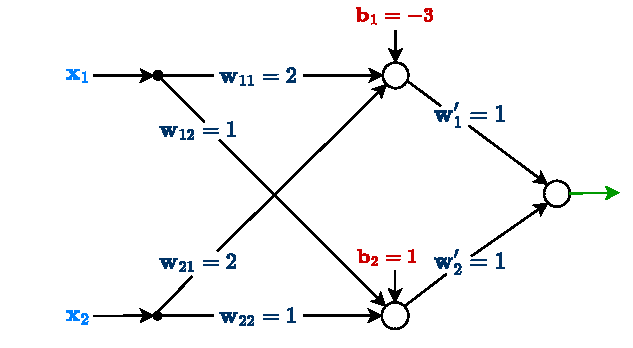
\includegraphics[width=1.\linewidth]{fig/1.pdf}
 \caption{\emph{Attribution shift} in a neural network with one hidden layer and ReLU activation functions. If $x_1=x_2=1$, both neurons of the hidden layer are activated, and the two inputs contribute to the output from both the upper and lower path. But, if $x_1=1, x_2=0$, the upper neuron of the hidden layer is deactivated, thus input $x_1$ cannot contribute from the upper path. It now contributes less to the model decision, leading to a drop in its attribution score.}
 \label{fig:simple-dnn}
\end{figure}
%------------------------------------------------------------------------------

The attribution shift and the OOD problem can also be observed by visual inspection of the attribution maps for different methods. A notable instance where heuristic techniques fail is when essential objects are segmented in more than one part, in which case the attribution one part may be suppressed by another, depending on how the background is masked. This scenario illustrated in \autoref{fig:or-blk-blr}, where both attribution shift and OOD occur.

\textbf{How can we hide information without attribution shift and without generating OOD images?} The authors of~\citep{Izzo_2021} suggest a pivotal insight: That the hiding process should depend not only on the input image, but also on the \emph{model parameters}. What we argue in this work is that this idea may help in addressing attribution shift, but to adress OOD, the hiding process must also depend on the entire \emph{data distribution} where the model is trained.

%------------------------------------------------------------------------------
\begin{figure}[t]
\newcommand{\sizeS}{.24}
\newcommand{\sizeP}{.165}
\newcommand{\hh}{.215\textwidth}
\newcommand{\ww}{.250\textwidth}
\setlength{\tabcolsep}{0pt}
\renewcommand{\arraystretch}{.2}
\centering
\footnotesize
\begin{tabular}{ccccc}
	& Original & Black & Blurry & ZIP (ours) \\
	\rotatebox{90}{~Image} & 
	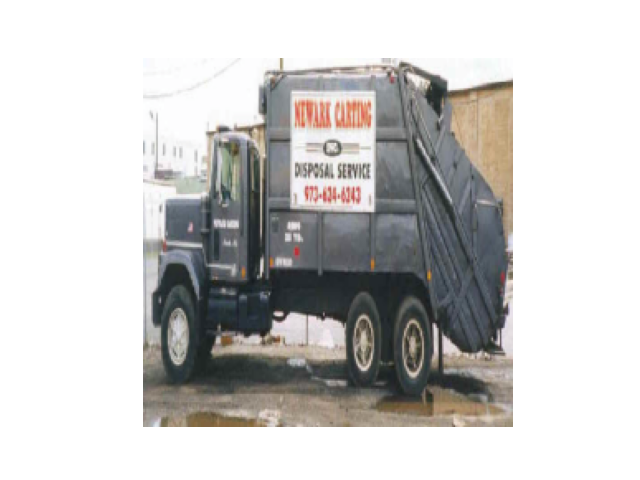
\includegraphics[trim={28mm 10mm 39mm 10mm},clip,width=\sizeS\linewidth]{fig/7_207/image.png} & 
	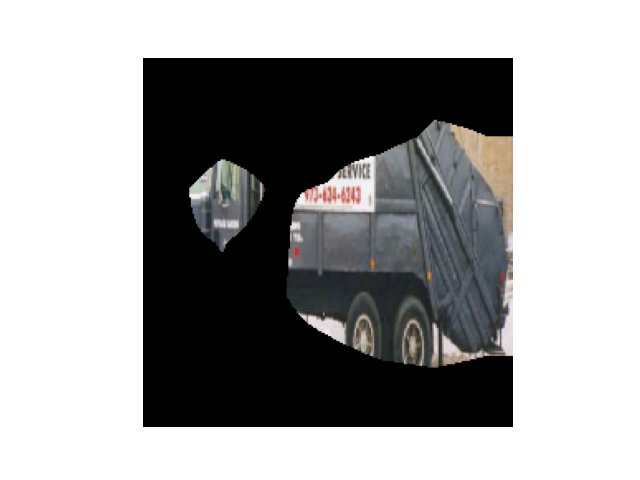
\includegraphics[trim={28mm 10mm 39mm 10mm},clip,width=\sizeS\linewidth]{fig/7_207/black_image.png} & 
	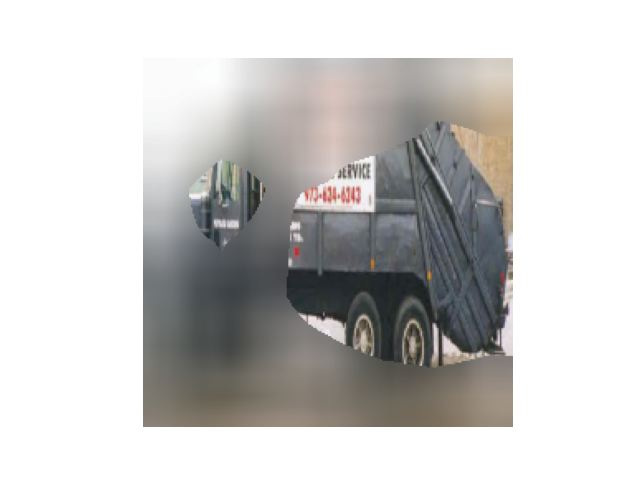
\includegraphics[trim={28mm 10mm 39mm 10mm},clip,width=\sizeS\linewidth]{fig/7_207/blurry_image.png} &
	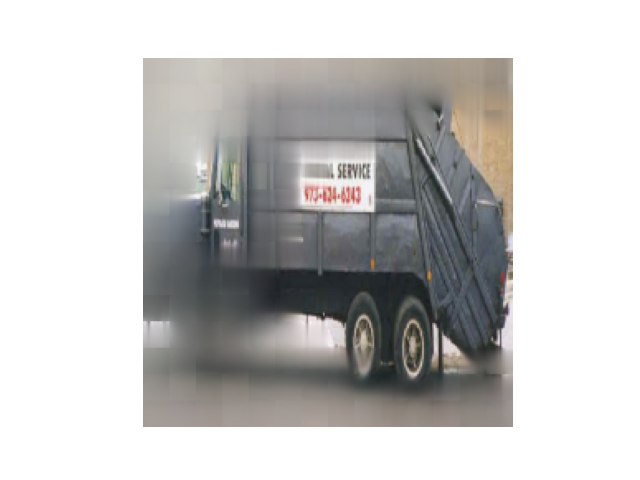
\includegraphics[trim={28mm 10mm 39mm 10mm},clip,width=\sizeS\linewidth]{fig/7_207/zip.png} \\
	\rotatebox{90}{~Attribution} &
	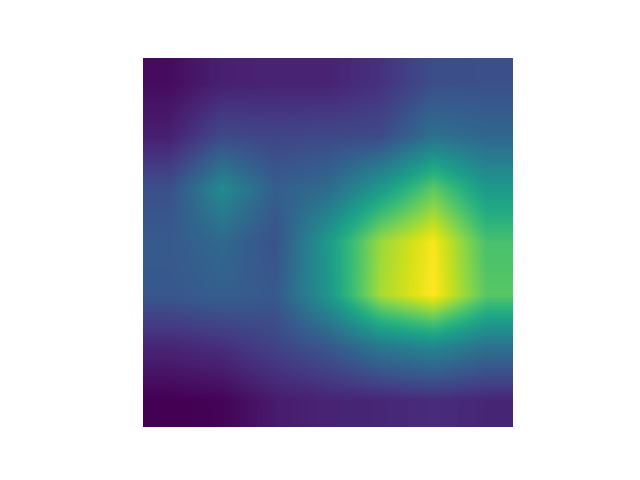
\includegraphics[trim={28mm 10mm 39mm 10mm},clip,width=\sizeS\linewidth]{fig/7_207/0.png} &
	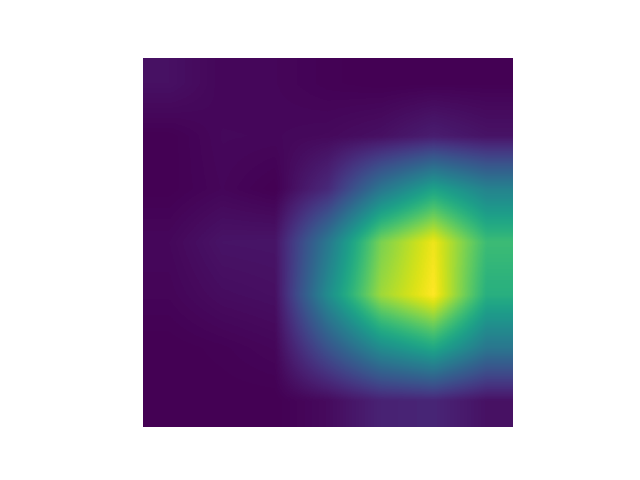
\includegraphics[trim={28mm 10mm 39mm 10mm},clip,width=\sizeS\linewidth]{fig/7_207/1.png} &
	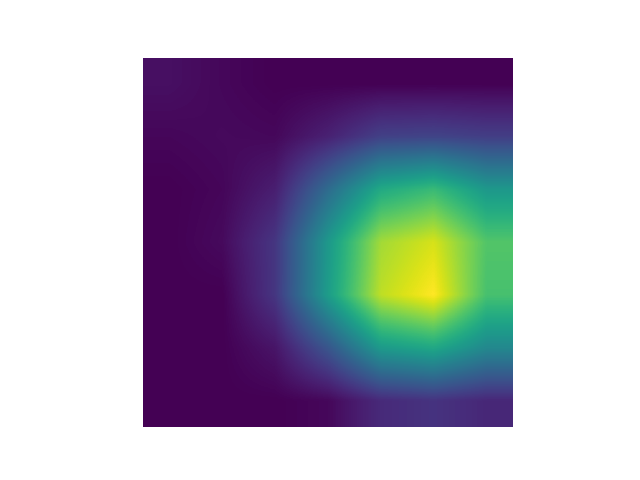
\includegraphics[trim={28mm 10mm 39mm 10mm},clip,width=\sizeS\linewidth]{fig/7_207/2.png} &
	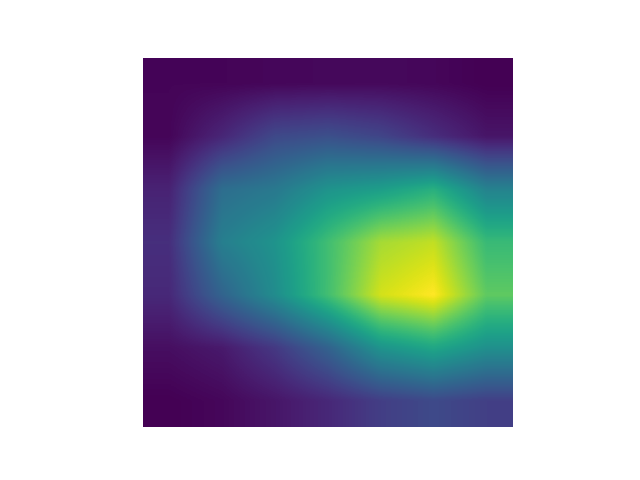
\includegraphics[trim={28mm 10mm 39mm 10mm},clip,width=\sizeS\linewidth]{fig/7_207/zip_attr.png} \\
\end{tabular}
\caption{Heuristic methods for hiding image parts induce \emph{attribution shift} of the visible parts. (Top) The image is masked by thresholding the attribution map of GradCAM; (bottom) a new attribution map is obtained for the masked image. Masking by black or blurry overlays result in the smaller left segment of the object disappearing from the new attribution map, unlike ZIP. The AttMask score~\eq{attmask} for black, blurry and ZIP are respectively \alert{TODO}.}
\label{fig:or-blk-blr}
\end{figure}
%------------------------------------------------------------------------------
